\documentclass[tikz,convert={outfile=images/m-algebra-cats.png,density=1000}]{standalone}
\usepackage[build={latexoptions={-output-directory=latex/png}}]{standalone}
\tikzset{
  ->/.style={draw=white!50!black,-stealth}
}
\tikzstyle{every node}=[color=white!50!black,font=\footnotesize]
\begin{document}
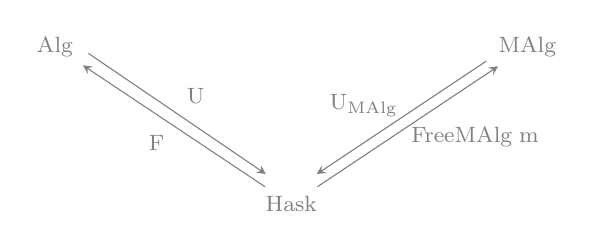
\begin{tikzpicture}
    \node (A) at (0,2) {\(\mathrm{Alg}\)};
    \node (B) at (6,2) {\(\mathrm{M\-Alg}\)};
    \node (C) at (3,0) {\(\mathrm{Hask}\)};
    \node (A') at (0.3, 2.0) {};
    \node (B') at (5.6, 1.9) {};
    \node (C') at (2.8, 0.3) {};
    \node (C'') at (3.2, 0.3) {};
    \draw [->] (A') -- node [above right] {\(\mathrm{U}\)} (C'); 
    \draw [->] (C) -- node [below left]   {\(\mathrm{F}\)} (A); 
    \draw [->] (C) -- node [above left]   {\(\mathrm{U}_{\mathrm{MAlg}}\)} (B);
    \draw [->] (B') -- node [below right] {\(\mathrm{FreeMAlg\; m}\)} (C'');
\end{tikzpicture}
\end{document}
